\documentclass[]{article}

% Margins
\addtolength{\oddsidemargin}{-.875in}
\addtolength{\evensidemargin}{-.875in}
\addtolength{\textwidth}{1.75in}
\addtolength{\topmargin}{-.875in}
\addtolength{\textheight}{1.75in}

% Math stuff
\usepackage{amsfonts}
\usepackage{amsmath}
\usepackage{amsthm}
\usepackage{cancel}
\usepackage{mathtools}

\newcommand{\transpose}{^{\top}}
\newcommand{\defeq}{\vcentcolon=}
\newcommand{\eqdef}{=\vcentcolon}

\newcommand*\circled[1]{\raisebox{.5pt}{\textcircled{\raisebox{-.9pt} {#1}}}}
\DeclareMathOperator*{\argmax}{arg\,max}
\DeclareMathOperator*{\argmin}{arg\,min}
\newcommand{\mat}[1]{\mathrm{\mathbf{#1}}}
\newcommand{\colvec}[1]{\mathbf{#1}}
\newcommand{\greekcolvec}[1]{\boldsymbol{#1}}
\newcommand{\mathcurs}[1]{\text{\calligra #1}}
\newcommand{\cframe}[1]{\left\{\mathrm{#1}\right\}}
\newcommand{\Ad}[1]{\left[\mathrm{Ad}_{T_\mathrm{#1}}\right]}
\newcommand{\ad}[1]{\left[\mathrm{ad}_{\mathcal{V}_\mathrm{#1}}\right]}

\theoremstyle{definition}
\newtheorem{definition}{Definition}[section]

\theoremstyle{remark}
\newtheorem*{remark}{Remark}

% Abbreviations and acronyms
\newcommand{\ie}{i.e., }
\newcommand{\eg}{e.g., }
\newcommand{\vs}{vs.\ }
\newcommand{\etal}{et al.}
\newcommand{\Poincare}{Poincar{\'e}}

\usepackage[nolist,nohyperlinks]{acronym}
\acrodef{BOA}[BOA]{basin of attraction }
\acrodef{COM}[COM]{center of mass }
\acrodef{DEM}[DEM]{discrete element method }
\acrodef{DOF}[DOF]{degree-of-freedom }
\acrodef{DOFs}[DOF]{degree of freedom }
\acrodef{GM}[GM]{granular media }
\acrodef{GRF}[GRF]{ground reaction force }
\acrodef{HZD}[HZD]{hybrid zero dynamics }
\acrodef{IMU}[IMU]{inertial measurement unit}
\acrodef{LCP}[LCP]{linear complementarity problem}
\acrodef{LO}[LO]{liftoff}
\acrodef{MRAC}[MRAC]{model reference adaptive control }
\acrodef{MPC}[MPC]{model predictive control}
\acrodef{NLP}[NLP]{nonlinear program}
\acrodef{ODE}[ODE]{ordinary differential equation }
\acrodef{PMP}[PMP]{Pontryagin's Maximum Principle }
\acrodef{RFT}[RFT]{resistive force theory }
\acrodef{RL}[RL]{reinforcement learning }
\acrodef{STC}[STC]{self-tuning control}
\acrodef{SLIP}[SLIP]{spring-loaded inverted pendulum }
\acrodef{SQP}[SQP]{sequential quadratic programming}
\acrodef{TD}[TD]{touchdown}
\acrodef{TPBVP}[TPBVP]{two-point boundary value problem}
\acrodef{ZMP}[ZMP]{zero-moment point }

% Graphics stuff
\usepackage{graphicx}
% \graphicspath{ {./graphics/eps/} }
\usepackage{caption}
\usepackage{subcaption}
\usepackage{epstopdf}

\usepackage{url}
\usepackage{hyperref}
\hypersetup{
	colorlinks=true,
	linkcolor=blue,
	filecolor=magenta,      
	urlcolor=blue,
}

\begin{document}

% \maketitle

% \begin{abstract}
% This document uses tools from modern robotics to develop a coordinate-free representation of the dynamics of a rigid body in state-space form: $\dot{\colvec{x}} = \colvec{f}\left(\colvec{x},\colvec{u}\right)$.
% \end{abstract}

% \tableofcontents
\section*{Geometric Integration with Event Detection for Simulating Coordinate-Free State-Space Rigid Body Dynamics with Impacts}
\noindent\hrule
\medskip
This repo is an extension of another repo I created, \href{https://github.com/dlynch7/geometric_rigid_body_dynamics}{\texttt{geometric\_rigid\_body\_dynamics}}, in which I demonstrated how a geometric integrator is used to simulate rigid body dynamics directly in terms of homogeneous transformation matrices, twists, and wrenches, without having to deal with multiple coordinate charts.

In this repo, I add two more features:
\begin{itemize}
	\item event detection: detects when the rigid body impacts the ground;
	\item impact map: updates the state of the rigid body after impact.
\end{itemize}

I came across a preprint of a similar paper: ``\href{https://mathweb.ucsd.edu/~mleok/pdf/TrLe2023_collisions.pdf}{Lie Group Variational Collision Integrators for a Class of Hybrid Systems}'' by Tran and Leok. It takes a slightly different approach to the problem but is a helpful reference!

\section{Hybrid Dynamics}
We model and simulate a bouncing ball as a hybrid system, \ie a system consisting of continuous dynamics (the differential equations of motion of the ball when in free fall) and discrete dynamics (the algebraic equations that relate the post-impact state of the ball to its pre-impact state).
At a high level of abstraction, the hybrid dynamics are
\begin{subequations}
\begin{align}
	\dot{x} &= f(x),\qquad\textrm{if }h(x) \neq 0,\\
	x^{+} &= \Delta(x^{-}),\qquad\textrm{if }h(x) = 0,
\end{align}
\end{subequations}
where $f$ is a vector field that defines the continuous-time dynamics, $h(x)$ is the \textit{event function} (a function of the state $x$ that returns zero when impact occurs) and $\Delta$ is a function that maps the pre-impact state $x^{-}$ to the post-impact state $x^{+}$.

In this repo, the event function $h$ will return the height above ground of the lowest point on the ball, and the impact map $\Delta$ will arise from conservation of momentum.
My focus in this repo is on how to incorporate event detection in a Runge-Kutta geometric integrator, rather than on the details of the event function, so I will start with a simple case: a spherical ball;
as such, the distance between the ground and the bottom of the ball is not affected by the ball's orientation.
Simulation of an ellipsoidal ball is likely to produce more interesting (maybe even chaotic!) results but I'll save that for later.

\subsection{Continuous Dynamics}
In this repo, I am using the geometric integrator proposed by \href{https://doi.org/10.1007/BF02429858}{Crouch and Grossman (J. Nonlinear Sci., 1993)} to simulate the motion of a rigid body in 3D space.
The body has 6 degrees of freedom (DOF), but in order to avoid the pitfalls associated with choosing a set of 6 generalized coordinates, I am using a coordinate-free approach by working directly with the 4x4 homogeneous transformation matrix that represents the body's configuration in space.

Denote this transformation matrix $T_\mathrm{wb}\in \mathbb{SE}(3)$, where $\left\{\mathrm{w}\right\}$ is the world frame and $\left\{\mathrm{b}\right\}$ is the body frame, i.e., a frame oriented along the body's principal axes of inertia and whose origin is located at the body's center of mass (COM).
The special Euclidean group $\mathbb{SE}(3)$ is a \textit{Lie group}---a kind of differentiable manifold that has special geometry that is not preserved by generic numerical integration algorithms like 4th-order Runge-Kutta, which operate on the $n$-dimensional Euclidean space $\mathbb{R}^n$.
Thus, a different approach is required to faithfully simulate coordinate-free rigid body dynamics. To do this, Crouch and Grossman propose a modified 4th-order Runge-Kutta scheme, which I'll call CG4.

Represented as a system of first-order ordinary differential equations (ODEs), the equations of motion for a rigid body in space are

\begin{equation}\label{eq:first_order_state_space_dynamics}
\frac{\mathrm{d}}{\mathrm{d}t}
\underbrace{
\begin{bmatrix}
T_\mathrm{wb}(t)\\
\mathcal{V}_\mathrm{b}(t)
\end{bmatrix}}_{x}
=
\underbrace{\begin{bmatrix}
T_\mathrm{wb}(t)\left[\mathcal{V}_\mathrm{b}(t)\right]\\
\mathcal{K}\left(t,T_\mathrm{wb}(t),\mathcal{V}_\mathrm{b}(t)\right)
\end{bmatrix}}_{f(x)},
\end{equation}
where
\begin{equation}
\mathcal{K}\left(t,T_\mathrm{wb}(t),\mathcal{V}_\mathrm{b}(t)\right) = \mathcal{G}_\mathrm{b}^{-1}\left(\left[\mathrm{ad}_{\mathcal{V}_\mathrm{b}(t)}\right]^{\top}\mathcal{G}_\mathrm{b}\mathcal{V}_\mathrm{b}(t) + \mathcal{F}_\mathrm{b}(t)\right).
\end{equation}
In these equations,
\begin{itemize}
	\item $T_\mathrm{wb}\in \mathbb{SE}(3)$ is the configuration of the body's COM frame $\left\{\mathrm{b}\right\}$ relative to the inertial world frame $\left\{\mathrm{w}\right\}$.
	\item $\left[\mathcal{V}_\mathrm{b}\right]\in\mathfrak{se}(3)$ is the matrix representation of the body twist $\mathcal{V}_\mathrm{b}\in\mathbb{R}^6$, where $\mathcal{V}_\mathrm{b} = \left[\omega_\mathrm{b}^{\top},v_\mathrm{b}^{\top}\right]^{\top}$, where $\omega_\mathrm{b}\in\mathbb{R}^3$ and $v_\mathrm{b}\in\mathbb{R}^3$ are the angular and linear velocity, respectively, represented in the COM frame $\left\{\mathrm{b}\right\}$.
	\item $\mathcal{G}_\mathrm{b}\in\mathbb{R}^{6\times6}$ is the body's inertia tensor; $\mathcal{G}_\mathrm{b}$ is a diagonal matrix with $\left(\mathcal{I}_{xx},\mathcal{I}_{yy},\mathcal{I}_{zz},\mathfrak{m},\mathfrak{m},\mathfrak{m}\right)$ along the diagonal, where $\mathcal{I}_{xx}$, $\mathcal{I}_{yy}$, and $\mathcal{I}_{zz}$ are the inertias about the principal axes and $\mathfrak{m}$ is the body's mass.
	\item $\mathcal{F}_\mathrm{b}\in\mathbb{R}^6$ is the net external wrench on the body, expressed in the COM frame. $\mathcal{F}_\mathrm{b} = \left[m_\mathrm{b}^{\top},f_\mathrm{b}^{\top}\right]^{\top}$, where $m_\mathrm{b}\in\mathbb{R}^3$ and $f_\mathrm{b}\in\mathbb{R}^3$ are the moment and force, respectively, in the COM frame.
	\item $\left[\mathrm{ad}_{\mathcal{V}_\mathrm{b}(t)}\right]$ is a 6x6 matrix used to express the rate of change of spatial momentum $\mathcal{P}_\mathrm{b} = \mathcal{G}_\mathrm{b}\mathcal{V}_\mathrm{b}$ due to the twist $\mathcal{V}_\mathrm{b}$.
\end{itemize}
Note that the state space of the first-order \ac{ODE} above is $\mathcal{X} = \mathbb{SE}(3)\times\mathbb{R}^6$, and the state $x\in\mathcal{X}$ is the pair $\left(T_\mathrm{wb},\mathcal{V}_\mathrm{b}\right)$.

\subsection{Discrete Dynamics}
\subsubsection{Event Function and Event Detection}
As stated above, our event function $h:\mathbb{SE}(3)\times\mathbb{R}^6 \to \mathbb{R}$ is the distance between the bottom of the ball and the ground.
If, while integrating Equation \eqref{eq:first_order_state_space_dynamics} from $t_k$ to $t_{k+1}$, we observe that $h(x(t_{k+1})) \neq h(x(t_k))$, we must find the event time $t_\mathrm{e}\in\left[t_k,t_{k+1}\right]$ such that $h(x(t_\mathrm{e}) = 0)$.

We consider two approaches to event finding:
\begin{itemize}
	\item Bisection root finding;
	\item Newton-Raphson root finding.
\end{itemize}
While the bisection method may take more iterations to converge to an acceptable estimate of $t_\mathrm{e}$, it is guaranteed to return an estimate in the time window $\left[t_k,t_{k+1}\right]$.
Conversely, while the Newton-Raphson method may be more elegant, it is possible it will return an estimate outside $\left[t_k,t_{k+1}\right]$, if $\mathrm{d}h/\mathrm{d}t$ is sufficiently small and $\mathrm{d}^2 h/\mathrm{d}t^2$ is sufficiently large.

\paragraph{Bisection Root Finding}
Searching for roots of the event function via bisection is simple:
\begin{enumerate}
	\item Given a time window $\left[t_k,t_{k+1}\right]$ for which $\mathrm{sign}(h(t_k)) \neq \mathrm{sign}(h(t_{k+1}))$, divide the time window in half to produce two new time windows: $\left[t_k, t_k + \Delta t/2\right]$ and $\left[t_k + \Delta t/2, t_{k+1}\right]$, where $\Delta t = t_{k+1} - t_k$.
	\item If $\mathrm{sign}(h(t_k)) \neq \mathrm{sign}(h(t_k + \Delta t/2))$, repeat step 1 for the new time window $\left[t_k, t_k + \Delta t/2\right]$. Otherwise, repeat step 1 for the new time window $\left[t_k + \Delta t/2, t_{k+1}\right]$.
	\item Iterate until some convergence criterion is satisfied, or until the maximum number of iterations is reached.
\end{enumerate}

\paragraph{Newton-Raphson Root Finding}
Given an initial guess at the event time $t_0\in\left[t_k,t_{k+1}\right]$, the Taylor series expansion of $h(x(t))$ at $t_{0}$ is
\begin{equation}
	h(x(t)) = h(x(t_0)) + \mathcal{L}_f h(x(t_0))\left(t - t_n\right) + \mathrm{h.o.t},
\end{equation}
where $\mathcal{L}_f h(x(t_0))$ is the Lie derivative of $h$ along $f$ evaluated at the state $x$ at time $t_0$:
\begin{align}
	\begin{split}
		\mathcal{L}_f h(x(t_0)) &= \frac{\mathrm{d}h}{\mathrm{d}t}\bigg\vert_{t_0}\\
		&= \frac{\partial h}{\partial x}\frac{\mathrm{d}x}{\mathrm{d}t}\bigg\vert_{t_0}\\
		&= \frac{\partial h}{\partial x}f(x(t_0)),
	\end{split}
\end{align}
where $f$ is the right-hand side of Equation \eqref{eq:first_order_state_space_dynamics}. 
Neglecting higher-order terms, setting $h(x(t)) = 0$, and solving for $t$, we obtain a first-order approximation for the event time:
\begin{equation}
	t \approx t_0 - \left(\mathcal{L}_f h(x(t_0))\right)^{-1}h(x(t_0)).
\end{equation}
Updating our initial guess with this new $t$ and repeating the above, we get the following iteration:
\begin{equation}
	t_{n+1} = t_{n} - \left(\mathcal{L}_f h(x(t_n))\right)^{-1}h(x(t_n)),
\end{equation}
which we repeat until some convergence criterion is satisfied or until the number of iterations reaches a user-specified maximum.

\paragraph{Simple Case - Sphere:}
The position of the bottom of a sphere with radius $r$ is
\begin{equation}
	h(T_\mathrm{wb},\mathcal{V}_\mathrm{b}) = a\transpose T_\mathrm{wb} b - r,
\end{equation}
where $a = \left[0,0,1,0\right]\transpose$ and $b = \left[0,0,0,1\right]\transpose$.
Intuitively, $\mathrm{d}h/\mathrm{d}t$ should be the velocity of the \ac{COM} in the $\hat{z}_\mathrm{w}$ direction: $\mathrm{d}h/\mathrm{d}t = a\transpose\dot{T}_\mathrm{wb} b$.
For this simple case,
\begin{equation}
	\frac{\partial h}{\partial T_\mathrm{wb}} = a b\transpose
	=
	\begin{bmatrix}
		0 & 0 & 0 & 0\\
		0 & 0 & 0 & 0\\
		0 & 0 & 0 & 1\\
		0 & 0 & 0 & 0
	\end{bmatrix}\textrm{ and }
	\frac{\partial h}{\partial \mathcal{V}_\mathrm{b}} = 0_{1\times 6}.
\end{equation}
It is worth noting that the 4-by-4 matrix above is $G_3$, one of the six generators of the Lie algebra $\mathfrak{se}(3)$:
\begin{align*}
	G_1 &= \begin{bmatrix}
		0 &0 &0 &1\\
		0 &0 &0 &0\\
		0 &0 &0 &0\\
		0 &0 &0 &0
	\end{bmatrix}, & 
	G_2 &= \begin{bmatrix}
		0 &0 &0 &0\\
		0 &0 &0 &1\\
		0 &0 &0 &0\\
		0 &0 &0 &0
	\end{bmatrix}, & 
	G_3 &= \begin{bmatrix}
		0 &0 &0 &0\\
		0 &0 &0 &0\\
		0 &0 &0 &1\\
		0 &0 &0 &0
	\end{bmatrix}, \\
	G_4 &= \begin{bmatrix}
		0 &0 &0 &0\\
		0 &0 &-1 &0\\
		0 &1 &0 &0\\
		0 &0 &0 &0
	\end{bmatrix}, & 
	G_5 &= \begin{bmatrix}
		0 &0 &1 &0\\
		0 &0 &0 &0\\
		-1 &0 &0 &0\\
		0 &0 &0 &0
	\end{bmatrix}, & 
	G_6 &= \begin{bmatrix}
		0 &-1 &0 &0\\
		1 &0 &0 &0\\
		0 &0 &0 &0\\
		0 &0 &0 &0
	\end{bmatrix}.
\end{align*}
This does indeed pull out just the $\hat{z}_\mathrm{w}$-component of $\dot{T}_\mathrm{wb}$, \ie the \ac{COM} velocity in the vertical direction.
It helps to think about the following pair of operators for ``unpacking'' a matrix into a vector and for ``packing'' a vector into a matrix:
\begin{align*}
	\mathrm{vec}: \mathbb{R}^{n\times m} \to \mathbb{R}^{nm},\\
	\mathrm{unvec}: \mathbb{R}^{nm} \to \mathbb{R}^{n\times m}.
\end{align*}
I will follow the row-major convention throughout this document, \ie
\begin{equation*}
	\mathrm{vec}\left(\begin{bmatrix}a_{11} & a_{12} \\ a_{21} & a_{22}\end{bmatrix}\right) = \begin{bmatrix} a_{11} & a_{12} & a_{21} & a_{22} \end{bmatrix}\transpose.
\end{equation*}
For our simple event function, $\mathrm{vec}\left(\partial h/\partial x\right) = \left[0_{1\times11}, 1, 0_{1\times 10}\right]$.

\paragraph{More Complex Case: Ellipsoid}
\begin{figure}
	\centering
	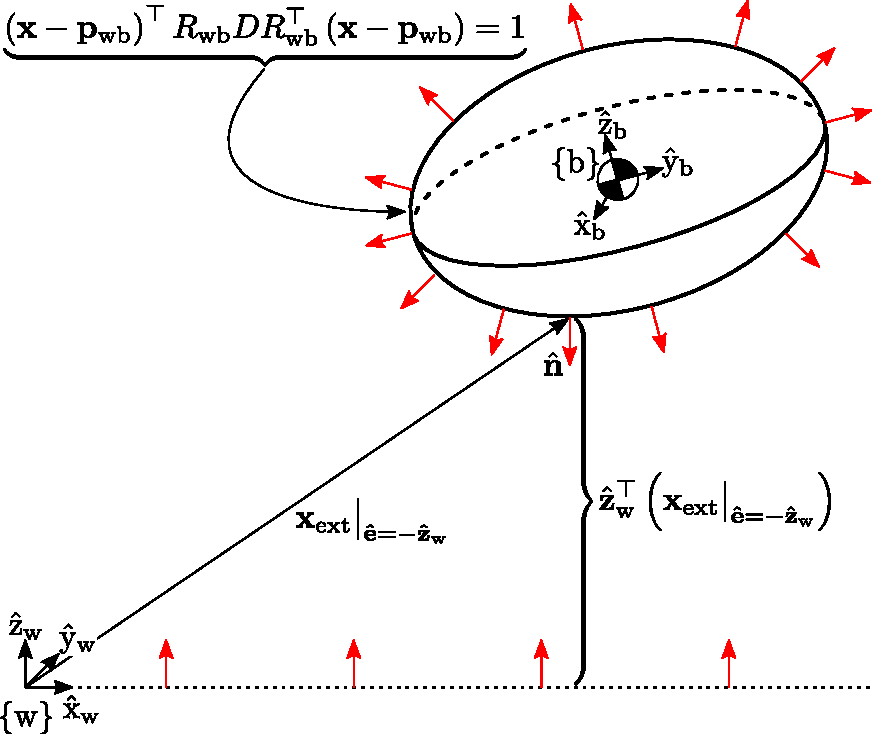
\includegraphics[width=0.66\linewidth]{graphics/pdf/ellipsoid_kinematics.pdf}
	\caption{Ellipsoid kinematics.
	The configuration of the ellipsoid is given by $T_\mathrm{wb}$.
	The lowest point on the ellipse, located at $\colvec{x}_\mathrm{ext}\big\vert_{\hat{\colvec{e}} = -\hat{\colvec{z}}_\mathrm{w}}$ in the $\cframe{w}$-frame, has unit surface normal $\hat{\colvec{n}}$, which points directly down.
	The distance from this point to the ground is given by the dot product of $\hat{\colvec{z}}$ and $\colvec{x}_\mathrm{ext}\big\vert_{\hat{\colvec{e}} = -\hat{\colvec{z}}_\mathrm{w}}$.}
	\label{fig:ellipsoid_kinematics}
\end{figure}
Suppose instead we want to know the distance between the lowest point on an ellipsoid and the ground, as shown in Figure \ref{fig:ellipsoid_kinematics}.
The ellipsoid is defined implicitly by the equation
\begin{equation}\label{eq:ellipsoid_implicit_Twb}
\left(\colvec{x} - \colvec{p}_\mathrm{wb}\right)\transpose R_\mathrm{wb} D R_\mathrm{wb}\transpose \left(\colvec{x} - \colvec{p}_\mathrm{wb}\right) = 1,
\end{equation}
where $\colvec{x}\in\mathbb{R}^3$, $\left(R_\mathrm{wb},\colvec{p}_\mathrm{wb}\right)\in\mathbb{SE}(3)$, and $D\in\mathbb{R}^{3\times 3}$ is a diagonal matrix whose entries are the reciprocals of the squares of the semi-axes.
For convenience, we will write \eqref{eq:ellipsoid_implicit_Twb} in the following more concise form:
\begin{equation}\label{eq:ellipsoid_implicit_simple}
	\colvec{y}\transpose A \colvec{y} = 1,
\end{equation}
where $\colvec{y} = \colvec{x} - \colvec{p}_\mathrm{wb}$ and $A = R_\mathrm{wb} D R_\mathrm{wb}\transpose$.
Note that $A$ is symmetric.
We will formulate the event function in a more general setting---how close is the ellipsoid to a (flat) surface whose unit normal vector is $\hat{\colvec{e}}$?---and we will then substitute the unit normal vector corresponding to level ground, $\hat{\colvec{e}} = -\hat{\colvec{z}}_\mathrm{w} = \left[0,0,-1\right]\transpose$.

For an ellipsoid, the unit vector normal to the surface at the point $\colvec{y}$ furthest in the $\hat{\colvec{e}}$-direction is simply $\hat{\colvec{e}}$.
The matrix $A$ in Equation \eqref{eq:ellipsoid_implicit_simple} stretches the vector $\colvec{y}$ by some amount $\mu$ and rotates it to align with $\hat{\colvec{e}}$:
\begin{equation}
	A\colvec{y} = \mu \hat{\colvec{e}}.
\end{equation}
Solving for $\colvec{y}$, we have
\begin{equation}\label{eq:furthest_point_on_ellipsoid_simple}
	\colvec{y} = \mu A^{-1}\hat{\colvec{e}}.
\end{equation}
Substituting this result into Equation \eqref{eq:ellipsoid_implicit_simple}, we have
\begin{align*}
	\begin{split}
		1 &= \colvec{y}\transpose A \colvec{y}\\
		&= \left(\mu A^{-1}\hat{\colvec{e}}\right)\transpose A \left(\mu A^{-1}\hat{\colvec{e}}\right)\\
		&= \mu^2 \hat{\colvec{e}}\transpose A^{-\top} A A^{-1} \hat{\colvec{e}}\\
		&= \mu^2 \hat{\colvec{e}}\transpose A^{-1} \hat{\colvec{e}}.
	\end{split}
\end{align*}
The simplification leading to the last line is possible because $A$ is symmetric.
Solving for the scaling factor $\mu$, we get
\begin{equation}
	\mu = \frac{1}{\sqrt{\hat{\colvec{e}}A^{-1}\hat{\colvec{e}}}}.
\end{equation}
Substituting this expression for $\mu$ into Equation \eqref{eq:furthest_point_on_ellipsoid_simple}, we get
\begin{equation}
	\colvec{y} = \frac{A^{-1}\hat{\colvec{e}}}{\sqrt{\hat{\colvec{e}}A^{-1}\hat{\colvec{e}}}}.
\end{equation}
We substitute $\colvec{x}_\mathrm{ext}\big\vert_{\hat{\colvec{e}}} - \colvec{p}_\mathrm{wb}$ for $\colvec{y}$ and $R_\mathrm{wb} D R_\mathrm{wb}\transpose$ for $A$ and solve for $\colvec{x}_\mathrm{ext}\big\vert_{\hat{\colvec{e}}}$, the world-frame position of the point on the ellipsoid that is farthest from the origin of $\cframe{w}$ in the $\hat{\colvec{e}}$-direction:
\begin{equation}\label{eq:furthest_point_on_ellipsoid_Twb}
	\colvec{x}_\mathrm{ext}\big\vert_{\hat{\colvec{e}}} = \colvec{p}_\mathrm{wb} + \frac{R_\mathrm{wb} D^{-1} R_\mathrm{wb}\transpose \hat{\colvec{e}}}{\sqrt{\hat{\colvec{e}}\transpose R_\mathrm{wb} D^{-1} R_\mathrm{wb}\transpose \hat{\colvec{e}}}}.
\end{equation}
Finally, to use Equation \eqref{eq:furthest_point_on_ellipsoid_Twb} to find the point on the ellipsoid closest to the ground, we substitute $\hat{\colvec{e}} = -\hat{\colvec{z}}_\mathrm{w}$ into Equation \eqref{eq:furthest_point_on_ellipsoid_Twb}.
The event function for the ellipsoid impacting ground is then
\begin{equation}
	h\left(T_\mathrm{wb},\mathcal{V}_\mathrm{b}\right) = \hat{\colvec{z}}_\mathrm{w}\transpose\left(\colvec{x}_\mathrm{ext}\big\vert_{\hat{\colvec{e}} = -\hat{\colvec{z}}_\mathrm{w}}\right) = 0.
\end{equation}

\subsubsection{Impact Map}
\end{document}